\chapter{球員程式碼}
\renewcommand{\baselinestretch}{10.0} %設定行距
\pagenumbering{arabic} %設定頁號阿拉伯數字
\setcounter{page}{4}  %設定頁數
\fontsize{14pt}{2.5pt}\sectionef
\section{車體改良-操作}
  為了增加對戰的刺激性及操作的方便性,我們對球員的程式碼新增可以前後移動並同時左右移動還有添加倒地翻身的功能。\\[1pt]

\section{移動操作-輪子旋轉}
\begin{figure}[hbt!]
\begin{center},
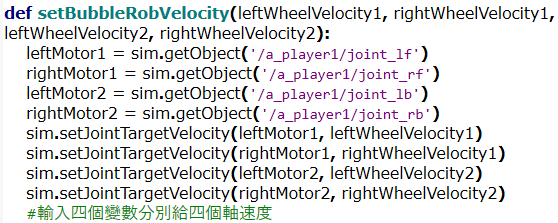
\includegraphics[height=6cm]{40}
\caption{\Large 設定球員輪子旋轉}\label{fig.40}
\end{center}
\end{figure}
(圖.\ref{40}) 設定一個 setVelocity 函數,接受四個參數:leftWheelVelocity1,rightWheelVelocity1,leftWheelVelocity2,rightWheelVelocity2,分別為左右前後輪速度。在函數內部使用 sim.getObject() 函數獲取左右前後輪的關節 joint ,並使用 sim.setJointTargetVelocity() 函數將各關節的目標速度設置為傳入的參數值,這樣做及可控制球員輪子速度,從而使球員移動。\\
\newpage
\section{移動操作-前輪方向}
\begin{figure}[hbt!]
\begin{center}
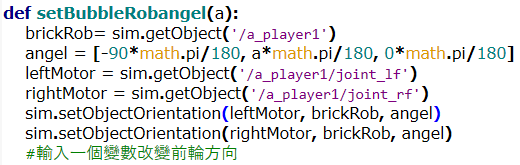
\includegraphics[height=4cm]{41}
\caption{\Large 設定球員前輪方向}\label{fig.41}
\end{center}
\end{figure}
(圖.\ref{41}) 設定一個 setBubbleRobange1 函數,接受一個設置角度值得參數 "a",以函數 sim.getObject 獲取一個代表 "a player"模型的對象"brickRob"。計算角度值並傳入參數"a"轉換為弧度值,將另兩個角度分別為固定角度值。在使用 sim.getObject() 獲取左右前輪的關節,以 sim.setObjectOrientation() 將關節地朝向設置為與 brickRob 相對應的角度,便可以給定角度旋轉並改變球員地朝向位置。\\
\section{移動操作-左右轉向}
\begin{figure}[hbt!]
\begin{center}
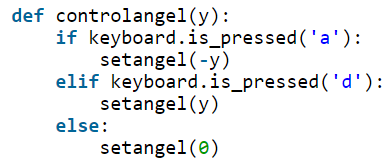
\includegraphics[height=4cm]{42}
\caption{\Large 控制球員左右轉向}\label{fig.42}
\end{center}
\end{figure}
(圖.\ref{42}) controlange1 函數接受控制角度的函數"y",檢查按鍵輸入,按下"a"調用 setangel(-y) ,將傳入函數取相反值設成角度;按下"d"則用 setangel(y),傳入函數直接設成角度;無按下任何鍵則調用 setangel(0),將角度設為零。\\
  此程式碼根據按鍵輸入來控制角度值輸入,可以分別控制向左向右角度值。\\
\section{移動操作-控制球員移動}
\begin{figure}[hbt!]
\begin{center}
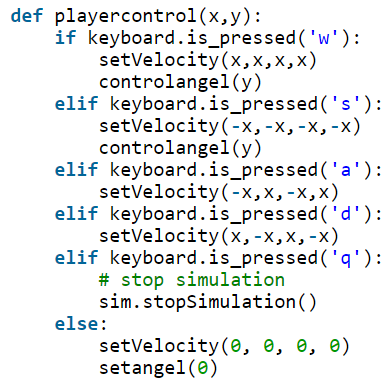
\includegraphics[height=8cm]{43}
\caption{\Large wasd移動球員}\label{fig.43}
\end{center}
\end{figure}
(圖.\ref{43}) 以 playcontrol 函數定義參數"x"和"y",代表速度及角度。檢查按鍵輸入,如果按下"w"將調用 setVelocity(x, x, x, x)設置輪子速度、調用 controlangel(y) 控制角度。若為 setVelocity(-x, -x, -x, -x)則設置為反向速度,按下"q"則停止模擬。\\
  根據鍵盤輸入 w, a, s, d 來控制球員前進、後退、左轉和右轉。\\
\newpage
\section{移動操作-維持速度}
\begin{figure}[hbt!]
\begin{center}
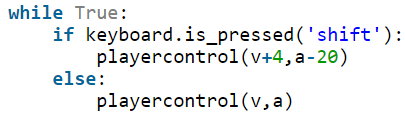
\includegraphics[height=3cm]{44}
\caption{\Large 控制球員速度}\label{fig.44}
\end{center}
\end{figure}
(圖.\ref{44}) 此程式碼使用無限循環"while True"迴圈,如果按下"shift"會調用 playcontrol(v+4, a-20)函數,使原有速度增加4,角度減去20。使用無線循環迴圈檢測鍵盤輸入,調整速度與角度。\\
\section{球員改良-倒地翻身}
\begin{figure}[hbt!]
\begin{center}
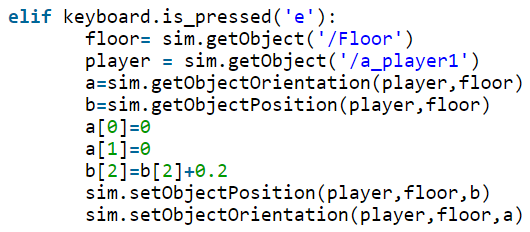
\includegraphics[height=5cm]{45}
\caption{\Large 控制球員翻身}\label{fig.45}
\end{center}
\end{figure}
(圖.\ref{45}) 定義如果按"e"就執行,以 sim.getObject('/Floor') 獲取地板句柄、('/a player1') 球員句柄;sim.getObjectOrientation(player,floor) 獲取相對於地板的球員方向、Position(player,floor) 獲取相對於地板的球員位置,將數值存於變量"a"及"b"中。a[0]=0 將球員的x角度為0,a[1]=0 將球員的y角度為0,b[2]=b[2]+0.2 將球員的z位置上升0.2。最後通過 sim.setObjectPosition(player,floor,b) 設定球員相對於地板的位置、Orientation(player,floor,a) 設定球員相對於地板的方向。\\
  此段程式碼根據按下"e"來執行將指定對象地朝向與位置進行修改,使球員翻倒後能夠再次翻身站起,繼續進行比賽。\\
\renewcommand{\baselinestretch}{1} %設定行距